% Preamble
% ---

% These are the instructions for authors for IJCAI-18.
% They are the same as the ones for IJCAI-11 with superficical wording
%   changes only.

\documentclass{article}
\usepackage{icml2018}
\usepackage{times}  %Required
\usepackage{helvet}  %Required
\usepackage{courier}  %Required
\usepackage{url}  %Required
\usepackage{graphicx}  %Required
\usepackage{titlesec}
\usepackage{mathtools}
\usepackage{comment}
\usepackage[11pt]{moresize}

\frenchspacing  %Required
\setlength{\pdfpagewidth}{8.5in}  %Required
\setlength{\pdfpageheight}{11in}  %Required
\setcounter{secnumdepth}{2}  
 
\titlespacing*{\paragraph}{0pt}{1.5ex plus 1ex minus .2ex}{1.3ex plus .2ex}
 
\usepackage{times}
\usepackage{xcolor}
\usepackage{soul}
%\usepackage[small]{caption}
\usepackage{nicefrac}
\usepackage{mathtools}

\usepackage{graphicx}
\usepackage{subfig}
\usepackage{caption}
% Packages
% ---
\usepackage{amsmath} % Advanced math typesetting
\usepackage{amssymb}
\usepackage{amsthm}
\usepackage{mathabx}
\usepackage{array}
\usepackage{bbm}
%\usepackage{subcaption}
\usepackage[ruled,linesnumbered,vlined]{algorithm2e}
%\usepackage{tikz}
%\usepackage{tkz-graph}
\usepackage{calrsfs}
%\usetikzlibrary{shapes,arrows,positioning,calc}
\usepackage[capitalize]{cleveref}

\crefname{algocf}{Algorithm}{Algorithm}
\Crefname{algocf}{Algorithm}{Algorithm}

\DeclarePairedDelimiter{\ceil}{\lceil}{\rceil}
\DeclarePairedDelimiter{\norm}{\lVert}{\rVert}
\DeclarePairedDelimiter{\abs}{\vert}{\rvert}

\makeatletter
\newcommand{\citeasnoun}[1]{\cite{#1}}
\newcommand*{\rom}[1]{\expandafter\@slowromancap\romannumeral #1@}
\makeatother
\newcommand{\E}{\mathbb{E}}
\renewcommand{\P}{\mathbb{P}}
\newcommand{\setsep}{~:~}
\newcommand{\opt}{^\star}
\newenvironment{mprog}{\begin{array}{>{\displaystyle}l>{\displaystyle}l>{\displaystyle}l}}{\end{array}}
\newcommand{\stc}{\\[1ex]  \mbox{s.t.} &}
\newcommand{\cs}{\\[1ex] & }
\newcommand{\minimize}[1]{\min_{#1} &}
\newcommand{\maximize}[1]{\max_{#1} &}
\newcommand{\tr}{^{\mathsf{T}}}
\newcommand{\one}{\mathbf{1}}
\newcommand{\Real}{\mathbb{R}}
\renewcommand{\ss}{~:~}

\newcommand{\eye}{\mathbf{I}}
\newcommand{\zero}{\mathbf{0}}

\usepackage{natbib}
\bibliographystyle{named}
\setcitestyle{square}

\newcommand{\RNum}[1]{\uppercase\expandafter{\romannumeral #1\relax}}
\newcommand*{\todo}{\textcolor{red}}
\newcommand{\marek}[1]{\textcolor{blue}{[[#1]]}}

\newcommand{\states}{\mathcal{S}}
\newcommand{\actions}{\mathcal{A}}
\newcommand{\tran}{p\opt}
\newcommand{\aset}{\mathcal{P}}
\newcommand{\aseth}{\aset^{H}}
\newcommand{\asetht}{\aset^{T}}
\newcommand{\asetb}{\aset^{B}}
\newcommand{\asetr}{\aset^{R}}
\newcommand{\BU}{T}
\newcommand{\rob}{^R}
\newcommand{\RBU}{\widehat{T}}
\newcommand{\indicator}{\mathbbm{1}}
\newcommand{\vset}{\mathcal{V}}
\newcommand{\vsetr}{\vset^R}

\newcommand{\statecount}{S}
\newcommand{\actioncount}{S}

%\newcommand{\fix}[1]{}
\newcommand{\fix}[1]{{$\langle${\color{red}\sc Fix: #1}$\rangle$}}

\theoremstyle{plain}
\newtheorem{theorem}{Theorem}[section]
\newtheorem{corollary}[theorem]{Corollary}
\newtheorem{lemma}[theorem]{Lemma}
\newtheorem{proposition}[theorem]{Proposition}
\theoremstyle{definition}
\newtheorem{definition}[theorem]{Definition}

\title{Robust Exploration with Tight Bayesian Plausibility Sets}
%PDF Info Is Required:
\pdfinfo{
	/Tight Bayesian Ambiguity Sets for Robust MDPs
	/author names}

\author{
UNH
}
\date{}
% Main document
% ---
\begin{document}
\maketitle

%\tikzset{
%block/.style = {draw, fill=white, rectangle, minimum height=3em, minimum width=3em},
%tmp/.style  = {coordinate}, 
%sum/.style= {draw, fill=white, circle, node distance=1cm},
%input/.style = {coordinate},
%output/.style= {coordinate},
%pinstyle/.style = {pin edge={to-,thin,black}}
%}

\begin{abstract}
Optimism about the poorly understood states and actions is the main driving force of exploration in provably-efficient reinforcement learning algorithms. We propose optimism in the face of sensible value functions (OFVF)- a novel reinforcement learning algorithm designed to explore robustly minimizing the worst case exploration cost, where the optimism is driven by tighter Bayesian bounds. OFVF proceeds in an episodic manner, where the duration of the episode is fixed and known. OFVF relaxes the requirement for the set of plausible MDPs to be represented by a confidence interval. It also optimizes the size and location of the plausibility set. Our algorithm is inherently Bayesian and can leverage prior information. Our theoretical analysis shows the robustness of OFVF, and the empirical results demonstrate its practical promise.
\end{abstract}

\section{Introduction}

Markov decision processes (MDPs) provide a versatile methodology for modeling dynamic decision problems under uncertainty~\citep{Bertsekas1996,Sutton1998,Puterman2005}. A perfect MDP model for many reinforcement learning problems is not known precisely in general. Instead, a reinforcement learning agent tries to maximize its cumulative payoff by interacting in an unknown environment with an effort to learn the underlying MDP model. It is important for the agent to explore
sub-optimal actions to accelerate the MDP learning task which can help to optimize long-term performance. But it is also important to pick actions with highest known rewards to maximize short-run performance. So the agent always needs to balance between them to boost the performance of a learning algorithm during learning. 

\emph{Optimism in the face of uncertainty (OFU)} is a common principle for most reinforcement learning algorithms encouraging exploration~\citep{Jaksch2010,Brafman2001,Kearns1998a}. The idea is to assign a very high exploration bonus to poorly understood states and actions. The agent chooses a policy under this very "optimistic" model of the environment. As the less understood states-actions are incentivized, they seem lucrative to the agent encouraging exploration. As the agent visits and gathers statistically significant evidence for these states-actions, the uncertainty and optimism decreases converging to reality. Many RL algorithms including \emph{Explicit Explore or Exploit $(E^3)$}~\citep{Kearns1998a}, \emph{R-{\ssmall MAX}}~\cite{Brafman2001}, \emph{UCRL2}~\cite{Auer2006} build on the idea of optimism guiding the exploration. These algorithms provide strong theoretical guarantees with polynomial bound on sample complexity. 

The performance of these OFU algorithms greatly depends on the methods to implement optimism, which can often be complex in nature. Dealing with a family of plausible environments can sometime become expensive as well. With OFU exploration, it is possible for an agent to end up in a catastrophic situation paying an extremely high price (e.g. a self driving car hits a wall, a robot falls off the cliff etc.). Exploring and learning such a situation may not payoff the price. It can be wise for the agent to be robust and avoid those situations minimizing the worst-case exploration cost$-$ which we call robust exploration. OFU algorithms are optimistic by definition and cannot guarantee robustness while exploring.

\emph{Probability matching} class of algorithms like \emph{Thompson sampling}~\citep{Thompson1933} performs exploration with a proportional likelihood to the underlying true parameters and has been successfully applied to multi-armed bandit problems~\citep{Agrawal2012,Agrawal2011}. \emph{Posterior Sampling for reinforcement learning (PSRL)}~\citep{Osband2016, Osband2013, Strens2002} applies the same idea in the context of reinforcement learning. PSRL algorithm samples a single instance of the environment from the posterior distribution, then solves and executes the policy optimal for that sampled environment over the episode. Selection of a policy in PSRL is proportional to the probability of that being optimal and exploration is guided by the variance of sampled policies as opposed to optimism. PSRL algorithm is simple, computationally efficient and can utilize any prior structural information to improve exploration. Strong theoretical analysis and practical applications for PSRL are also established in the literature. But similar to OFU algorithms, PSRL cannot handle worst case exploration penalty and performs poorly in such situations.

The main contribution of this paper is OFVF, a new \emph{data-driven} Bayesian approach to constructing \emph{Plausibility} sets for MDPs. The method computes policies with tighter robust estimates for exploration by introducing two new ideas. First, it is based on Bayesian posterior distributions rather than distribution-free bounds. Second, OFVF does not construct plausibility sets as simple confidence intervals. Confidence intervals as plausibility sets are a sufficient but not a necessary condition. OFVF uses the structure of the value function to optimize the \emph{location} and \emph{shape} of the plausibility set to guarantee upper bounds directly without necessarily enforcing the requirement for the set to be a confidence interval.

\section{Problem Statement}

We consider the problem of episodically learning and solving a 
finite-horizon MDP: $M = (S, A, P^M, R^M, H, \rho)$ where $S =
\{1,...,S\}$ is the state space, $A = \{1,...,A\}$ is the action
space,  $P^M(s'|s,a)$ is the believe distribution over the true
transition probability $P(s'|s,a)$ of transitioning to state $s'$ when
take action $a$ at state $s$, $R^M(s,a,s')$ is the believe
distribution over the true reward $R(s,a,s')$ when take action $a$ at
state $s$ and transition to state $s'$, $H$ is the time horizon, and
$\rho$ is the initial state distribution. In each episode, the initial
state $s_0$ is sampled from $\rho$, and in time period
$h=1,2,...,H$, if an action $a_h$ is taken in state $s_h$, then a
next state $s_{h+1}$ is sampled from $P(s_{h+1}|s_h,a_h)$ and a reward
$r_h$ is sampled from $R(s_h,s_a,s_{h+1})$. The episode terminates
when $s_H$ is reached. 

A policy $\mu$ is a function mapping $S$ to $A$. For each MDP $M$ and
policy $\mu$, we define a value function for each time period
$h=1,2,...,H$:

$V_h^\mu(s):=\mathbb{E}[\sum_{\tau=h}^H
r_\tau|s_h=s,a_\tau=\mu(s_\tau)]$

The optimal value function is
defined by $V^*_h(s)=\max_\mu V_h^\mu(s)$. A policy $\mu^*$ is said to
be optimal if $V^{\mu^*}=V^*$ for all $s\in S$ and $h=1,...,H$.

\fix{talk about state-action optimal value function? see RLSVI}

A reinforcement learning algorithm interacts with the MDP over
episodes from time period $\tau=1$ to $\tau=H$. At each time $\tau$,
the algorithm selects an action $a_\tau$, realizes a reward $r_\tau$,
and then transitions to state $s_{\tau+1}$. Over each episode $k$, the
algorithm realizes reward $\sum_{\tau=1}^H$. One way to quantify the
performance of a reinforcement algorithm is in terms of the expected
cumulative regret up to time $T$ over $K$ episodes, defined by

\begin{tabular}{l l l}
	$Regret(T,M)$ & $=$ &$
	\sum_{k=1}^{T/H}\mathbb{E}_M[V_1^*(s_{k1})-\sum_{\tau=1}^Hr_{k\tau}]$\\
	&$=$&$ \sum_{k=1}^{T/H}\mathbb{E}_M[V_1^*(s_{k1})-V_1^{\mu_k}(s_{k1})]$
\end{tabular}

\section{Bayesian Optimism in the Face of Uncertainty}

\begin{itemize}
	\item \todo{Talk a little about UCRL}
	\item \todo{explain the idea of Bayes UCRL}
	\item \todo{Explain why it outperforms UCRL (using variance of the distribution instead of distribution free Hoeffding bound )}
	\item \todo{Explain why it doesn't outperform PSRL (Rectangularity)}
\end{itemize}


\begin{algorithm}
	\KwIn{Desired confidence level $\delta$ and prior distribution }
	\KwOut{Policy with an optimistic return estimate }
	\Repeat{num episodes}{
		
		Initialize MDP: $M$\;
		Compute posterior: $\tilde{p} \gets$ compute\_posterior(prior, samples) \;
		
		\ForEach{$s \in \mathcal{S}, a \in \mathcal{A}$}{%
			$\bar{p}_{s,a}, \psi_{s,a} \gets$ Invoke Algorithm \ref{alg:bayes} with $\tilde{p}$, $\delta$\;
			$M \gets \text{add transition with } \bar{p}_{s,a}, \psi_{s,a}$\;
		}
		Compute policy by solving MDP: $\hat{\pi} \gets$ Solve $M$\;
		Collect samples by executing the policy: samples $\gets$ execute $\hat{\pi}$\;
		prior $\gets$ posterior\;
	}
	\Return $(\pi_k, p_0\tr v_k)$ \;
	\caption{Bayes UCRL}    \label{alg:IAVF}
\end{algorithm}

\section{OFVF: Optimism in the Face of sensible Value Functions} \label{sec:multiple}

OFVF uses samples from a posterior distribution, similar to a Bayesian confidence interval, but it relaxes the safety requirement as it is sufficient to guarantee for each state $s$ and action $a$ that:
\begin{equation} \label{eq:condition_safe}
\max_{v\in\mathcal{V}} \P_{P\opt} \left[ \min_{p \in \aset_{s,a}} (p - p_{s,a}\opt)\tr v \le 0  ~\middle|~ \mathcal{D} \right] \ge 1-\frac{\delta}{SA}~,
\end{equation}
with $\mathcal{V} = \{ \hat{v}\opt_{\aset} \}$. To construct the set $\aset$ here, the set $\mathcal{V}$ is not fixed but depends on the robust solution, which in turn depends on $\aset$. RSVF starts with a guess of a small set for $\mathcal{V}$ and then grows it, each time with the current value function, until it contains $\hat{v}\opt_{\aset}$ which is always recomputed after constructing the ambiguity set $\aset$.

\begin{algorithm}
	\KwIn{Desired confidence level $\delta$ and posterior distribution $\P_{P\opt}[\cdot ~|~\mathcal{D}]$ }
	\KwOut{Policy with a maximized safe return estimate }
	Initialize current policy $\pi_0 \gets \arg\max_{\pi} \rho(\pi,\E_{P\opt}[P\opt~|~\mathcal{D}])$\;
	Initialize current value $v_0 \gets v^{\pi_0}_{\E_{P\opt}[P\opt~|~\mathcal{D}]}$\;
	Initialize value robustness set $\mathcal{V}_0 \gets \{v_0 \}$ \;	
	\label{line:make_p_1} Construct $\aset_0$ optimal for $\mathcal{V}_0$\;
	Initialize counter $k\gets 0$\;
	\While{\cref{eq:condition_safe} is violated with $\mathcal{V}=\{v_k\}$}{
		Include $v_k$ that violates \cref{eq:condition_safe}: $\vset_{k+1} \gets \vset_k \cup \{ v_k \}$ \;
		\label{line:make_p_2} Construct $\aset_{k+1}$ optimized for $\vset_{k+1}$\;
		Compute robust value function $v_{k+1}$ and policy $\pi_{k+1}$ for $\aset_{k+1}$\;
		$k \gets k + 1$ \;
	}
	\Return $(\pi_k, p_0\tr v_k)$ \;
	\caption{OFVF: Optimism in the Face of sensible Value Functions}    \label{alg:IAVF}
\end{algorithm} 

In lines 4 and 8 of \cref{alg:IAVF}, $\aset_i$ is computed for each state-action $s,a \in \states\times\actions$. Center $\bar{p}$ and set size $\psi_{s,a}$ are computed from \cref{eq:center_point} using set $\mathcal{V}$ \& optimal $g_v$ computed by solving \cref{eq:optimal_hyperplane}.
When the set $\mathcal{V}$ is a singleton, it is easy to compute a form of an optimal ambiguity set. 
\begin{equation} \label{eq:optimal_hyperplane}
g = \max \left\{ k ~:~ \P_{P\opt} [k \le v\tr p\opt_{s,a}] \ge 1 - \delta/(SA) \right\}
\end{equation}

When $\mathcal{V}$ is a singleton, it is sufficient for the ambiguity set to be a subset of the hyperplane $\{ p \in \Delta^S ~:~ v\tr p = g\opt \}$ for the estimate to be safe. When $\mathcal{V}$ is not a singleton, we only consider the setting when it is discrete, finite, and relatively small. We propose to construct a set defined in terms of an $L_1$ ball with the minimum radius such that it is safe for every $v\in\mathcal{V}$. Assuming that $\mathcal{V} = \{v_1, v_2, \ldots, v_k \}$, we solve the following linear program:
\begin{equation} \label{eq:center_point}
\begin{gathered}
\psi_{s,a} = \min_{p\in\Delta^S} \Bigl\{ \max_{i=1,\ldots,k} \norm{q_i - p}_1 ~:~ 
\hspace{0.1cm}  v_i\tr  q_i = g_i\opt, q_i \in \Delta^S, i \in 1,\ldots,k  \Bigr\}
\end{gathered}
\end{equation}

In other words, we construct the set to minimize its radius while still intersecting the hyperplane for each $v$ in $\mathcal{V}$. \cref{alg:IAVF}, as described, is not guaranteed to converge in finite time as written. It can be readily shown the value functions in the individual iterations are non-increasing. It is easy to just stop once the value function becomes smaller (and that is more conservative) than BCI.

\begin{figure}
	\centering
	\begin{minipage}[c]{.45\columnwidth}
		\centering
		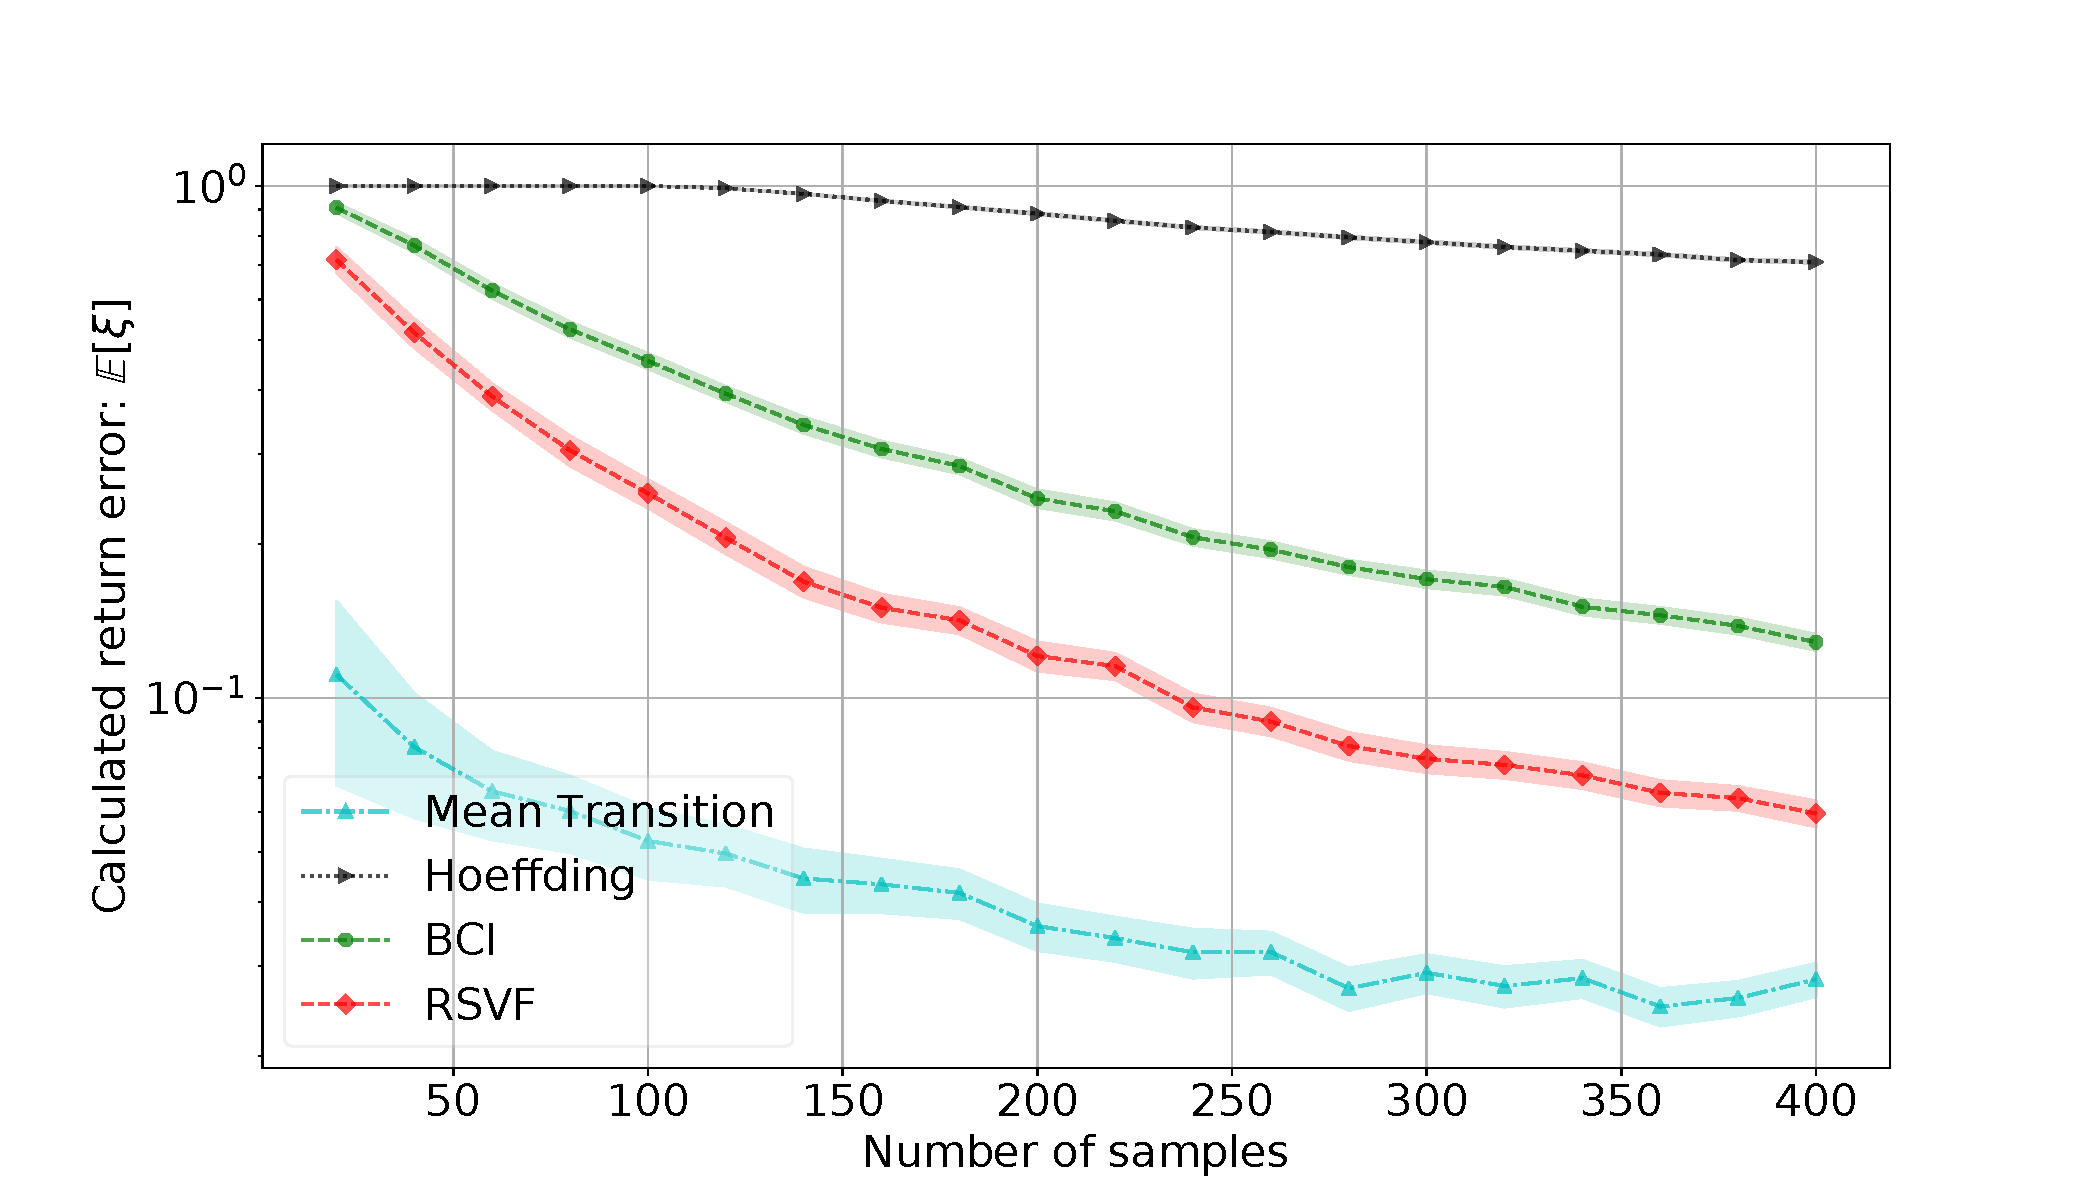
\includegraphics[width=\linewidth]{fig/gaussian_return_single_state.pdf}\\
	\end{minipage}%
	\begin{minipage}[c]{.45\columnwidth}
		\centering
		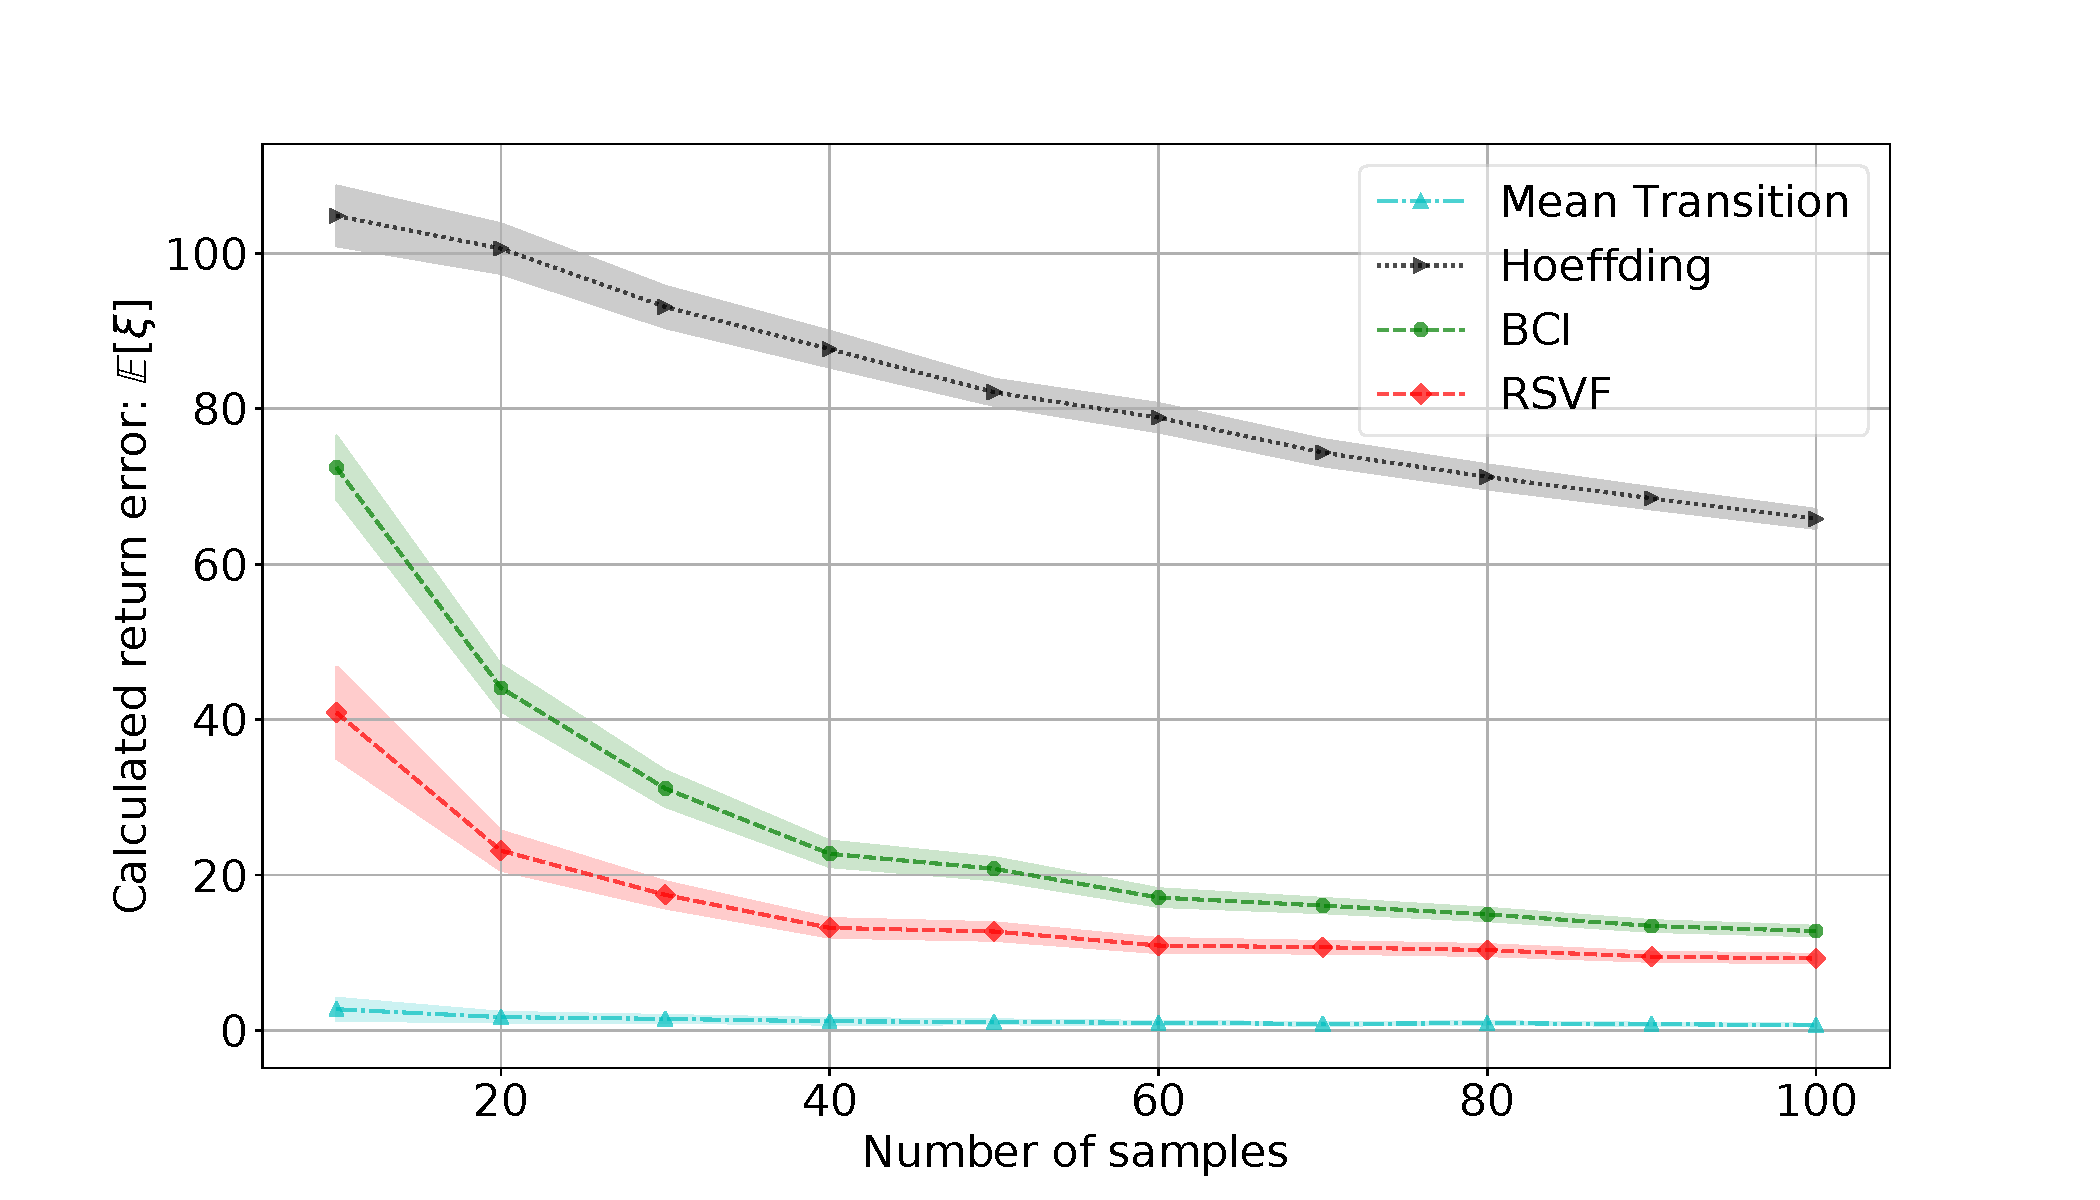
\includegraphics[width=\linewidth]{fig/Glossy_Buckthorn_Under_Estimation.pdf}
	\end{minipage}%
	\caption{Return error with a Gaussian prior with 95\% confidence, Left: Single state, Right: Full MDP, X-axis is the number of samples per state-action.}
	\label{fig:return_single_multiple}
\end{figure}

\section{Empirical Evaluation} \label{sec:experiments}

In this section, we evaluate the worst-case estimates computed by Bayes UCRL and OFVF empirically. We assume a true model of each problem and generate a number of simulated data sets for the known distribution. We compute the tightest optimistic estimate for the optimal return and compare it with the optimal return for the true model. We compare our results with ``UCRL2`` and ``PSRL`` algorithms. The value $\xi$ represents the predicted regret, which is the absolute difference between the \emph{true} optimal value and the robust estimate: $\xi = \abs{\rho(\pi\opt_{P\opt}, P\opt) - \hat\rho(\hat\pi\opt)}$, a smaller regret is better. All of our experiments use a 95\% confidence for safety unless otherwise specified.

\subsection{Single-state Bellman Update}
We initially consider simple problems where transition from a single non-terminal state following a single action leads to multiple terminal states. The value function for the terminal states are fixed and assumed to be provided. We evaluate different priors over the transition probabilities: i) uninformative Dirichlet prior and ii) informative Gaussian prior. Note that RSVF is optimal in this simplistic setting, as \cref{fig:dirichlet_result} (left) and \cref{fig:return_single_multiple} (left) shows. As expected, the mean estimate provides the tightest bound, but \cref{fig:dirichlet_result} (right) illustrates that it does not provide any meaningful safety guarantees.

\subsection{River Swim Problem}

\subsection{Mountain Car Problem}


\bibliography{marek,reazul_lib}

\newpage
\appendix
\onecolumn

\section{Technical Results} \label{app:proofs}

\subsection{Computing Bayesian Confidence Interval}
\begin{algorithm}
	\KwIn{Distribution $\theta$ over $p\opt_{s,a}$, confidence level $\delta$, sample count $m$}
	\KwOut{Nominal point $\bar{p}_{s,a}$ and $L_1$ norm size $\psi_{s,a}$}
	Sample $X_1, \ldots, X_m \in \Delta^S$ from $\theta$: $X_i \sim \theta $\;
	Nominal point: $\bar{p}_{s,a} \gets (1/ m) \sum_{i=1}^m X_i $\;
	Compute distances $d_i \gets \lVert \bar{p}_{s,a} - X_i \rVert_1$ and sort \emph{increasingly}\;
	Norm size: $\psi_{s,a} \gets d_{(1-\delta)\,m}$\;
	\Return{$\bar{p}_{s,a}$ and $\psi_{s,a}$}\;
	\caption{Bayesian Confidence Interval (BCI)} \label{alg:bayes}
\end{algorithm}

\end{document}
